\documentclass[a4paper,11pt,ngerman]{scrartcl}
\usepackage{babel}
\usepackage[T1]{fontenc}
\usepackage[utf8x]{inputenc}
\usepackage[a4paper,margin=2.0cm,footskip=1.0cm]{geometry}
\usepackage{wrapfig}
%\usepackage[english]{babel} 
\usepackage{verbatim}
\usepackage{tcolorbox}


% Die nächsten vier Felder bitte anpassen:
\newcommand{\Aufgabe}{Aufgabe 4: Würfelglück } % Aufgabennummer und Aufgabennamen angeben
\newcommand{\TeamId}{?????}                       % Team-ID aus dem PMS angeben
\newcommand{\TeamName}{234bcd}                 % Team-Namen angeben
\newcommand{\Namen}{Michael Köhler}           % Namen der Bearbeiter/-innen dieser Aufgabe angeben
 
% Kopf- und Fußzeilen
\usepackage{scrlayer-scrpage, lastpage}
\setkomafont{pageheadfoot}{\large\textrm}
\lohead{\Aufgabe}
\rohead{Team-ID: \TeamId}
\cfoot*{\thepage{}/\pageref{LastPage}}

% Position des Titels
\usepackage{titling}
\setlength{\droptitle}{-1.0cm}

% Für mathematische Befehle und Symbole
\usepackage{amsmath}
\usepackage{amssymb}

% Für Bilder
\usepackage{graphicx}
\graphicspath{ {./images/} }

% Für Algorithmen
%\usepackage{algpseudocode}

% Für Quelltext

\usepackage{listings}
\usepackage{color, colortbl}
\definecolor{mygreen}{rgb}{0,0.6,0}
\definecolor{mygray}{rgb}{0.5,0.5,0.5}
\definecolor{mymauve}{rgb}{0.58,0,0.82}
 \definecolor{cloudwhite}{rgb}{0.225, 0.225, 0.204} 
\definecolor{red}{rgb}{0.4,0,0} 
\definecolor{blue}{rgb}{0,0,0.6}
\definecolor{green}{rgb}{0,0.6,0}
\definecolor{cyan}{rgb}{0.0,0.6,0.6}
\lstset{
language=csh,
basicstyle=\footnotesize\ttfamily,
numbers=left,
numberstyle=\tiny,
numbersep=5pt,
tabsize=2,
extendedchars=true,
breaklines=true,
frame=tb,
showspaces=false,
showtabs=false,
xleftmargin=17pt,
framexleftmargin=17pt,
framexrightmargin=5pt,
framexbottommargin=4pt,
showstringspaces=false,
% confing for comments
commentstyle=\color{green},
morecomment=[l]{//}, 
morecomment=[s]{/*}{*/}, 
% keywords for classes
morekeywords={  List, Program,MatchResult,MatchUp,Player,Random,Console,File,for },
keywordstyle=\color{cyan},
identifierstyle=\color{cloudwhite},
% keywords for types
emph={int,char,double,float,unsigned,void,bool,var,string,private,static,new,class,using,true,false,null},
emphstyle={\color{blue}},
% other keywords to highlight
classoffset=1, 
otherkeywords={throw,return,break},
morekeywords={throw,return,break},
keywordstyle=\color{mymauve},
classoffset=0,
% style for strings
stringstyle=\color{red}\ttfamily,
}
\tcbset{colframe=cloudwhite!50!cloudwhite,colupper=red!50!black,
	fonttitle=\bfseries,nobeforeafter,center title}


% Diese beiden Pakete müssen zuletzt geladen werden
%\usepackage{hyperref} % Anklickbare Links im Dokument
\usepackage{cleveref}

% Daten für die Titelseite
\title{\textbf{\Huge\Aufgabe}}
\author{\LARGE Team-ID: \LARGE \TeamId \\\\
	    \LARGE Team-Name: \LARGE \TeamName \\\\
	    \LARGE Bearbeiter*innen dieser Aufgabe: \\ 
	    \LARGE \Namen\\\\}
\date{\LARGE\today}


\begin{document}


\maketitle
\tableofcontents

\vspace{0.5cm}


\section{Lösungsidee}

 \begin{wrapfigure}{r}{0.3\textwidth} 
 	\centering
 	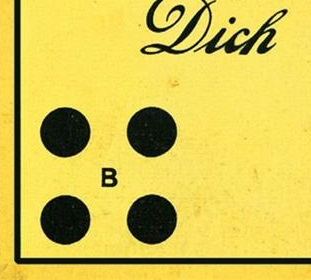
\includegraphics[width=0.11\textwidth]{home}	 	
 	\caption{B-Felder}
 	\label{fig:B-Felder}
 \end{wrapfigure}
Da die Beispielaufgaben unterschiedliche Spieler anzahlen enthalten, muss die Aufgabenstellung in drei
Teillaufgen unterteilt werden:

\begin{enumerate}
	
	\item Bestimmung der Spieler mit verwendeten Würfeln aus der gegebenen .txt Datei. Sowie das Erstellen von Paarungen.
	\item \glqq Spielen\grqq\space von Partien in Ausreichender Menge um den besseren Würfel in der Paarung zu bestimmen.
	\item Vergleich von den Ergebnissen der einzelnen Partien um den besten Würfel von allen gegeben Würfeln zu Bestimmen.	
\end{enumerate}
Die Eigentliche Logik der Aufgabe befindet sich im zweiten Punkt. Hier müssen die Gegeben Regeln des Mensch ärgere dich nicht Spiels berücksichtigt werden. Die hierbei wichtigsten Regeln sind:\\
\begin{wrapfigure}{r}{0.4\textwidth} 
	\centering
	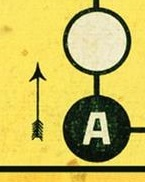
\includegraphics[width=0.15\textwidth]{start}	
	\caption{Startfeld/ A-Feld}
	\label{fig:Startfeld}
\end{wrapfigure}

\begin{wrapfigure}{r}{0.45\textwidth} 
	\centering
	
\includegraphics[width=0.1\textwidth]{goal}		
	\caption{Zielfelder [a, b, c, d]}
	\label{fig:Zielfelder}
\end{wrapfigure}
\begin{enumerate}
	
	\item [$\bullet$] Bei einer gewürfelten Sechs darf erneut gewürfelt werden.
	\item [$\bullet$]Bei einer Sechs wird falls möglich eine eigene Figur auf das Feld A (Abbildung \ref{fig:Startfeld}) der eigenen Farbe gestellt.
	\item [$\bullet$] Eine Gegnerische Figur die das Feld besetzt wird beim betreten geschlagen (zurück auf eines der B Felder).
	\item [$\bullet$] Die vorderste Figur wird immer als erstes versucht zu bewegen (Abweichung von den Offiziellen Regel)
	\item [$\bullet$] Die Zielfelder [a, b, c, d] (Abbildung \ref{fig:Zielfelder}) müssen genau erreicht werden. Es dürfen keine \glqq Augenzahlen \grqq\space verfallen
	\item [$\bullet$] Kann die vorderste Figur nicht bewegt werden, wird so lange die nächste weiteste Figur versucht zu bewegen.
	\item [$\bullet$] Kann keine der Figuren auf der \glqq Laufbahn\grqq \space bewegt werden, verfällt der Zug.
	\item [$\bullet$] Felder auf denen eine eigene Figur steht können nicht betreten werden. Auf den Zielfeldern dürfen eigene Figuren nicht übersprungen werden.
	\item [$\bullet$] Die Spieler führen ihre Züge immer im wechsel aus.
\end{enumerate}


\section{Umsetzung}
 
Die Lösungsidee wird in \texttt{C\#} implementiert. Spieler, Spielfiguren und Spielfeld lassen sich sehr gut als Objekte einfach nachvollziehbar darstellen, daher biete sich für die Aufgabe ein Objektorientierte Sprache an.
\subsection{Erstellung der Spiele /\glqq Matche\grqq} 
Für die Ermittlung der \glqq Matche\grqq wird die Textdatei ausgelesen und für jede Zeile ein Spieler erstellt mit dem entsprechenden Würfel als Array von Integer. Jeder Spieler wird in einer 2 Dimensionalen Matrix mit jedem Spieler gepaart (Tabelle \ref{table:Matrix}).
\begin{wraptable}{r}{8cm}	
	\centering
	\begin{tabular}{|c|c|c|c|c|}	
		\hline
		& Spieler 1 & Spieler 2 & Spieler 3 & Spieler 4\\
		\hline
		Spieler 1 &\cellcolor{mygray}& 2/1 & 3/1 & 4/1 \\	
		\hline
		Spieler 2 & 1/2 & \cellcolor{mygray} & 3/2 & 4/2 \\
		\hline
		Spieler 3 & 1/3 & 2/3 &\cellcolor{mygray}& 4/3 \\
		\hline
		Spieler 4 & 1/4 & 2/4 & 3/4 & \cellcolor{mygray} \\
		\hline
	\end{tabular}
	\caption{Matrix für Matches}
	\label{table:Matrix}
\end{wraptable}
Spiele gegen sich selbst werden dabei ignoriert. Dadurch wird sicher gestellt, dass jeder Spieler zweimal gegen jeden Anderen Spieler antritt (Hin- und Rückrunde mit getauschten Seiten). Die Matrix wird mit Hilfe einer doppelten foreach() Schleife erstellt, die für jeden Spieler Spiele erstellt (für jeden eins).
\subsection{Ausführung der \glqq Matche\grqq}
Für Jedes Match werden nun so lange \glqq Spiele\grqq \space gespielt, bis ein eindeutiger Sieger der beiden Spieler zu erkennen ist. Als ausreichende Menge von Spielen werden 40 festgelegt. Um die Laufzeit des Programms zu optimieren, wird bei einen bestimmten Verhältnis von Siegen das Match vorzeitig beendet:
\begin{enumerate}
	\item[$\bullet$] Vier Siege ohne gegen Sieg.	
	\item[$\bullet$] Ein Verhältnis von größer 4:1 bei bis zu 10 Spielen insgesamt.
	\item[$\bullet$] Ein Verhältnis von größer 2:1 bei über 10 Spielen. 
\end{enumerate}
\subsection{Spielen der \glqq Spiele\grqq}
Die Laufbahn wird über ein eindimensionales Array von Integer dargestellt. Jeder der Beiden Spieler erhält die Eigenschaften:
\begin{enumerate}
	\item[$\bullet$] Spielfiguren (Mit Eigenschaft Position als Integer)
	\item[$\bullet$] Startfeld (\glqq A Felder\grqq) je nach Spieler 1 oder 21.
	\item[$\bullet$] \glqq Zieleingang\grqq \space je nach Spieler 20 oder 40 als Abzweigung zu den Zielfeldern.	
\end{enumerate} 
Bis einer der Spieler alle Figuren auf den Zielfeldern stehen hat, führen beide im Wechsel je immer einen Zug aus.
\subsection{Durchführen eines Zugs}


 

\section{Beispiele}
\subsection{wuerfel0.txt}
Eingabe:

\begin{tcolorbox}[center,width=12cm,title=Textfiles/wuerfel0.txt]
	\centering
	\verbatiminput{Textfiles/wuerfel0.txt}
\end{tcolorbox}
Ausgabe:
\verbatiminput{Textfiles/wuerfel0_result.txt}
\subsection{wuerfel1.txt}
Eingabe:
\verbatiminput{Textfiles/wuerfel1.txt}
Ausgabe:
\verbatiminput{Textfiles/wuerfel1_result.txt}
\subsection{wuerfel2.txt}
Eingabe:
\verbatiminput{Textfiles/wuerfel2.txt}
Ausgabe:
\verbatiminput{Textfiles/wuerfel2_result.txt}
\subsection{wuerfel3.txt}
Eingabe:
\verbatiminput{Textfiles/wuerfel3.txt}
Ausgabe:
\verbatiminput{Textfiles/wuerfel3_result.txt}
\section{Quellcode}
%Unwichtige Teile des Programms sollen hier nicht abgedruckt werden. Dieser Teil sollte nicht mehr als 2–3 Seiten umfassen, maximal 10.
Beispiel-Code:
\begin{lstlisting}
static void Main(string[] args)
        {
//test Comment!
            List<Player> players = SetPlayers(args);
            List<MatchUps> matchups = CreateMatchups(players);
            List<GameResults> gameresults = PlayGames(matchups);
            RankPlayers(gameresults);
	 Console.WriteLine("Test string");
            
        }
\end{lstlisting}
Program.cs:
\lstinputlisting{DiceCompare/Program.cs}

\end{document}
